\documentclass{article}
\usepackage{graphicx,fancyhdr,amsmath,amssymb,amsthm,subfig,url,hyperref}
\usepackage[margin=1in]{geometry}
\usepackage{xltxtra}
\usepackage{xgreek}
\usepackage{amsfonts}
\usepackage{listings}
\usepackage{amssymb}
\usepackage{amsmath}
\usepackage{pdfpages}
\setmainfont[Mapping=tex-text]{Times New Roman}
%----------------------- Macros and Definitions --------------------------

%% FILL THIS OUT
\newcommand{\studentname}{Νικόλαος Ζαρίφης}
\newcommand{\suid}{03112178}
\newcommand{\exerciseset}{ SET 2}
%% END



\renewcommand{\theenumi}{\bf \Alph{enumi}}

%\theoremstyle{plain}
%\newtheorem{theorem}{Theorem}
%\newtheorem{lemma}[theorem]{Lemma}

\fancypagestyle{plain}{}
\pagestyle{fancy}
\fancyhf{}
\fancyhead[RO,LE]{\bfseries\large NTUA}
\fancyhead[LO,RE]{\bfseries\large Στοχαστικές Ανελίξεις}
\fancyfoot[LO,RE]{\bfseries\large \studentname: nick.zarifis@hotmail.com}
\fancyfoot[RO,LE]{\bfseries\thepage}
\renewcommand{\headrulewidth}{1pt}
\renewcommand{\footrulewidth}{1pt}

\graphicspath{{figures/}}

%-------------------------------- Title ----------------------------------

\title{Στοχαστικές Ανελίξεις\\ \exerciseset}
\author{\studentname \qquad  ID: \suid}

%--------------------------------- Text ----------------------------------

\begin{document}
\maketitle
\section*{Άσκησή 1}
\begin{itemize}
	\item i Βλέπουμε γραμμή γιατί ο οριζόντιος άξωνας είναι ως προς $logx$ άρα είναι σαν να έχουμε την έυθεια : y= 5 + 3x
	\item ii
		Γραφικά βλέπουμε πως η κλήση τις είναι μεγαλύτερη του 10/4 .
	\item iii Δεν αλλάζει σχεδόν κάθολου πέρα από μετακίνηση δηλάδη να έχει αυξηθεί η σταθερά β τις $y=ax+b$.
	\item iv
		Εδώ αλλάζει μόνο η κλίση τις εύθειας από ότι βλέπουμε.
	\item v
		Το αποτέλεσμα ήταν:The fitted line is y=(3.00)*x+(5.00) . Όποτε ναι συμφώνει με τα παραπάνω.

\end{itemize}
\section*{Άσκησή 2}
\begin{itemize}
	\item i
		Χώρις καμία αλλαγή τα αποτελέσματα αλλάζουν αρκέτα. ΠΧ.
	 9.5,9.938 και 10.188 .Αν μέγαλοσουμε το N έχουμε:
	 \begin{lstlisting}
In this experiment with    64 iterations, our Monte Carlo estimator of 
the mean duration of an excursion around state '1' is 11.859
In this experiment with   128 iterations, our Monte Carlo estimator of 
the mean duration of an excursion around state '1' is 9.641
In this experiment with   256 iterations, our Monte Carlo estimator of
 the mean duration of an excursion around state '1' is 10.047
In this experiment with   512 iterations, our Monte Carlo estimator of
 the mean duration of an excursion around state '1' is 10.717
In this experiment with  1024 iterations, our Monte Carlo estimator of
 the mean duration of an excursion around state '1' is 10.607
In this experiment with  2048 iterations, our Monte Carlo estimator of
 the mean duration of an excursion around state '1' is 10.276
In this experiment with  4096 iterations, our Monte Carlo estimator of
 the mean duration of an excursion around state '1' is 10.666

	 \end{lstlisting}
Δηλάδη όσο μεγαλώνει το Ν φτάνει κοντά στα 10 με 11 βήματα.Αλλά ακόμα έχουμε αποκλείσεις .
\item ii
	Βάζοντας τα ακόλουθα: 
	\begin{lstlisting}
	mcestimates = list()
	for k in xrange(30):
	mcestimates.append(MCestimate)

	\end{lstlisting}
	Πετυχαίνουμε το αποτέλεσμα μας. 
\item iii
	 \begin{lstlisting}

	for N= 64 sample mean: 10.252604 and sample variance:0.332083
	for N= 128 sample mean: 10.713802 and sample variance:0.084420
	for N= 256 sample mean: 10.447786 and sample variance:0.125896
	for N= 512 sample mean: 10.488737 and sample variance:0.063916
	for N= 1024 sample mean: 10.465332 and sample variance:0.030340
	for N= 2048 sample mean: 10.508789 and sample variance:0.016344
\end{lstlisting}
\item iv 

	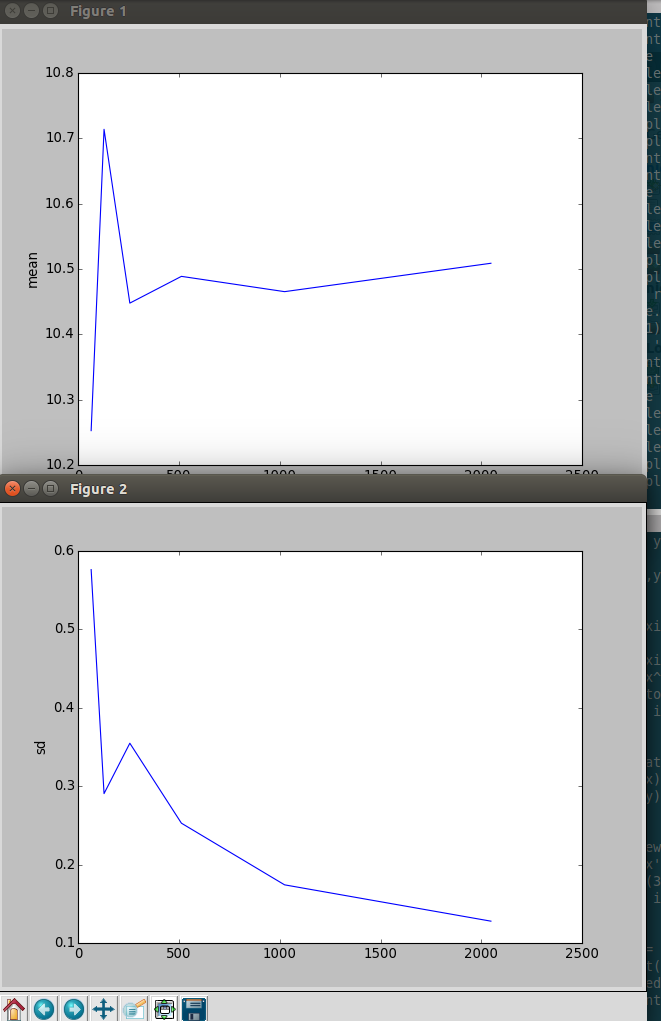
\includegraphics[height=200pt,width=150pt]{plot1}
\item v
	Για να το ύπολογίσουμε θεωρήτικα κατασκευάζουμε τις γραμμικές εξισώσεις:(πινακας μεταβασεις απο προγραμμα python).
$k_1 =0$, $k_2 = 0.3 k_3 + 0.6 k_4+1$,$k_3=0.8k_3+1+0.2k_5$,$k_4=1+0.5k_4 + 0.5k_5$, $k_5=0.2k_1+0.8k_5$ .Η λύση είναι: 
$k_2=9$,$k_3=10$,$k_4=7$ και $k_5=5$ άρα ο αναμενόμενος χρόνος είανι: $0.5 k_2 + 0.5 k_3 = 10.5$. Συμφωνεί με την προσομοίωση μας.
\ item vi 
		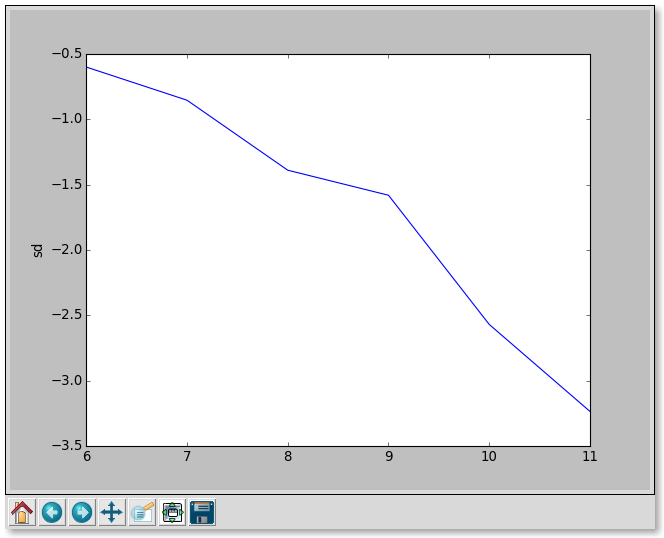
\includegraphics[height=200pt,width=200pt]{plot2}
		Ταιριάζοντας με ένα πολύωνημο 1ου βαθμού βλέπουμε πως η κλήση είναι: -0.56.
 \end{itemize}
\section*{Άσκησή 3}
Ακολουθόντας τα βήματα έχουμε τις ακόλουθα στιγμιότυπα: 
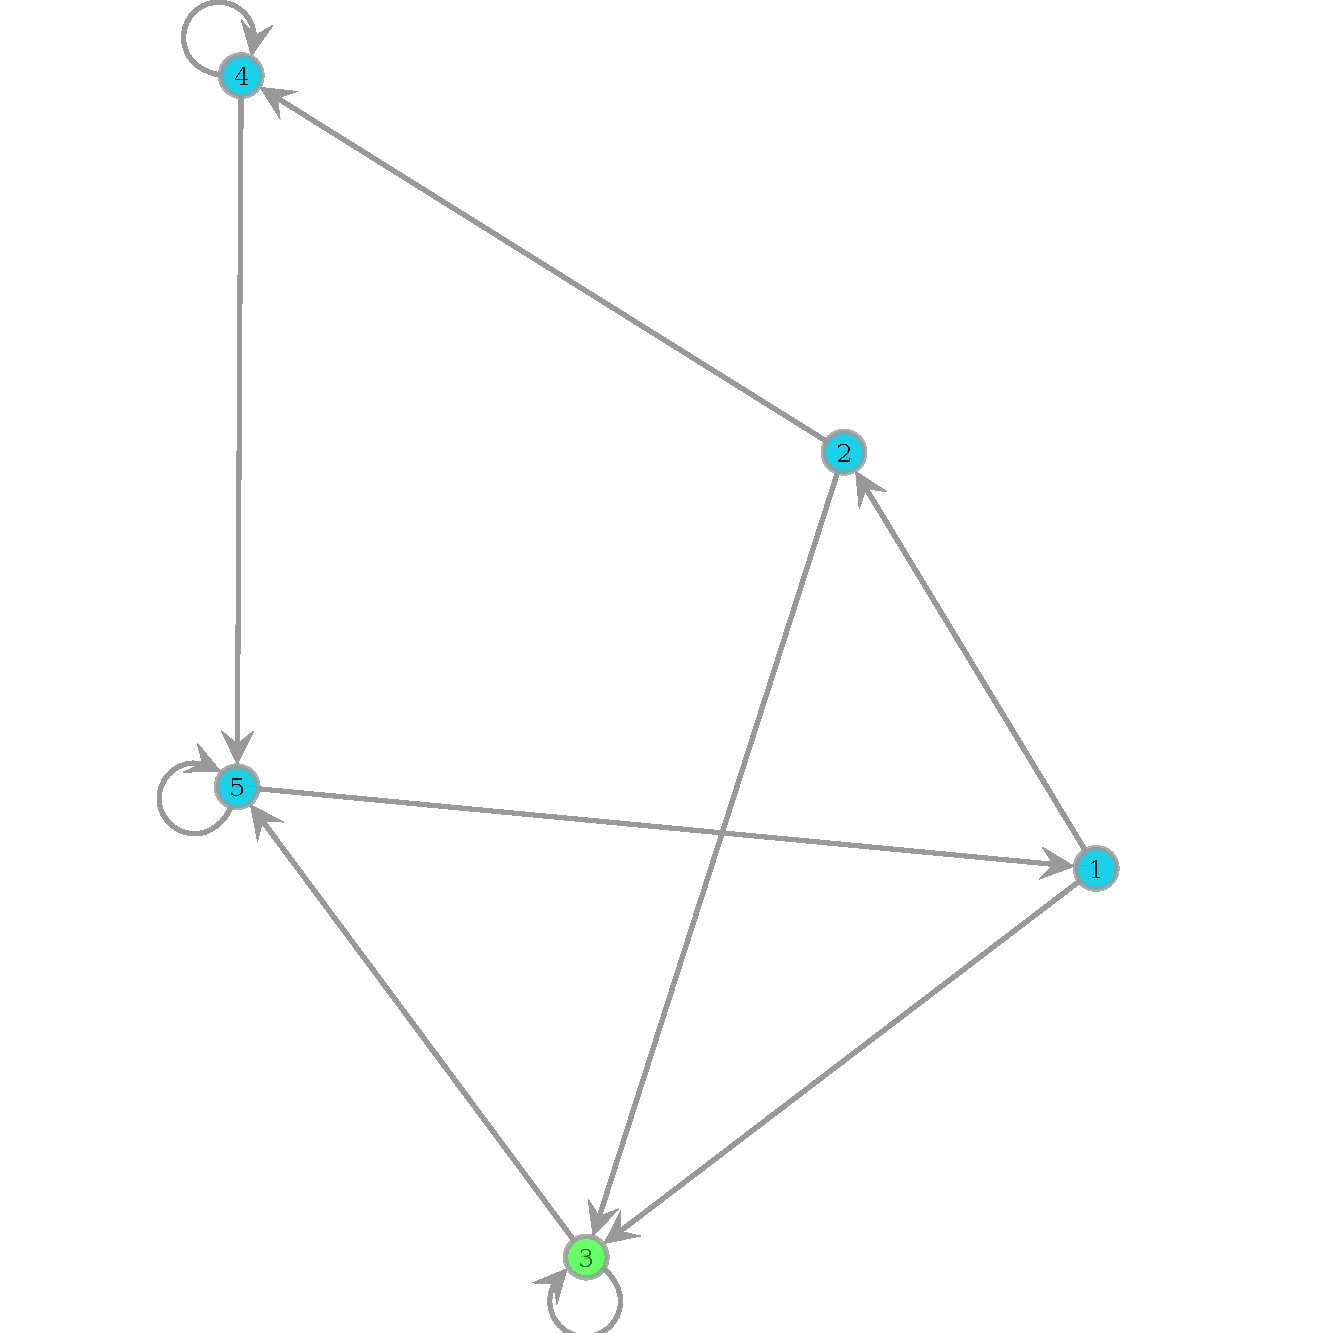
\includepdf[pages={1}]{mc_frame1.pdf}
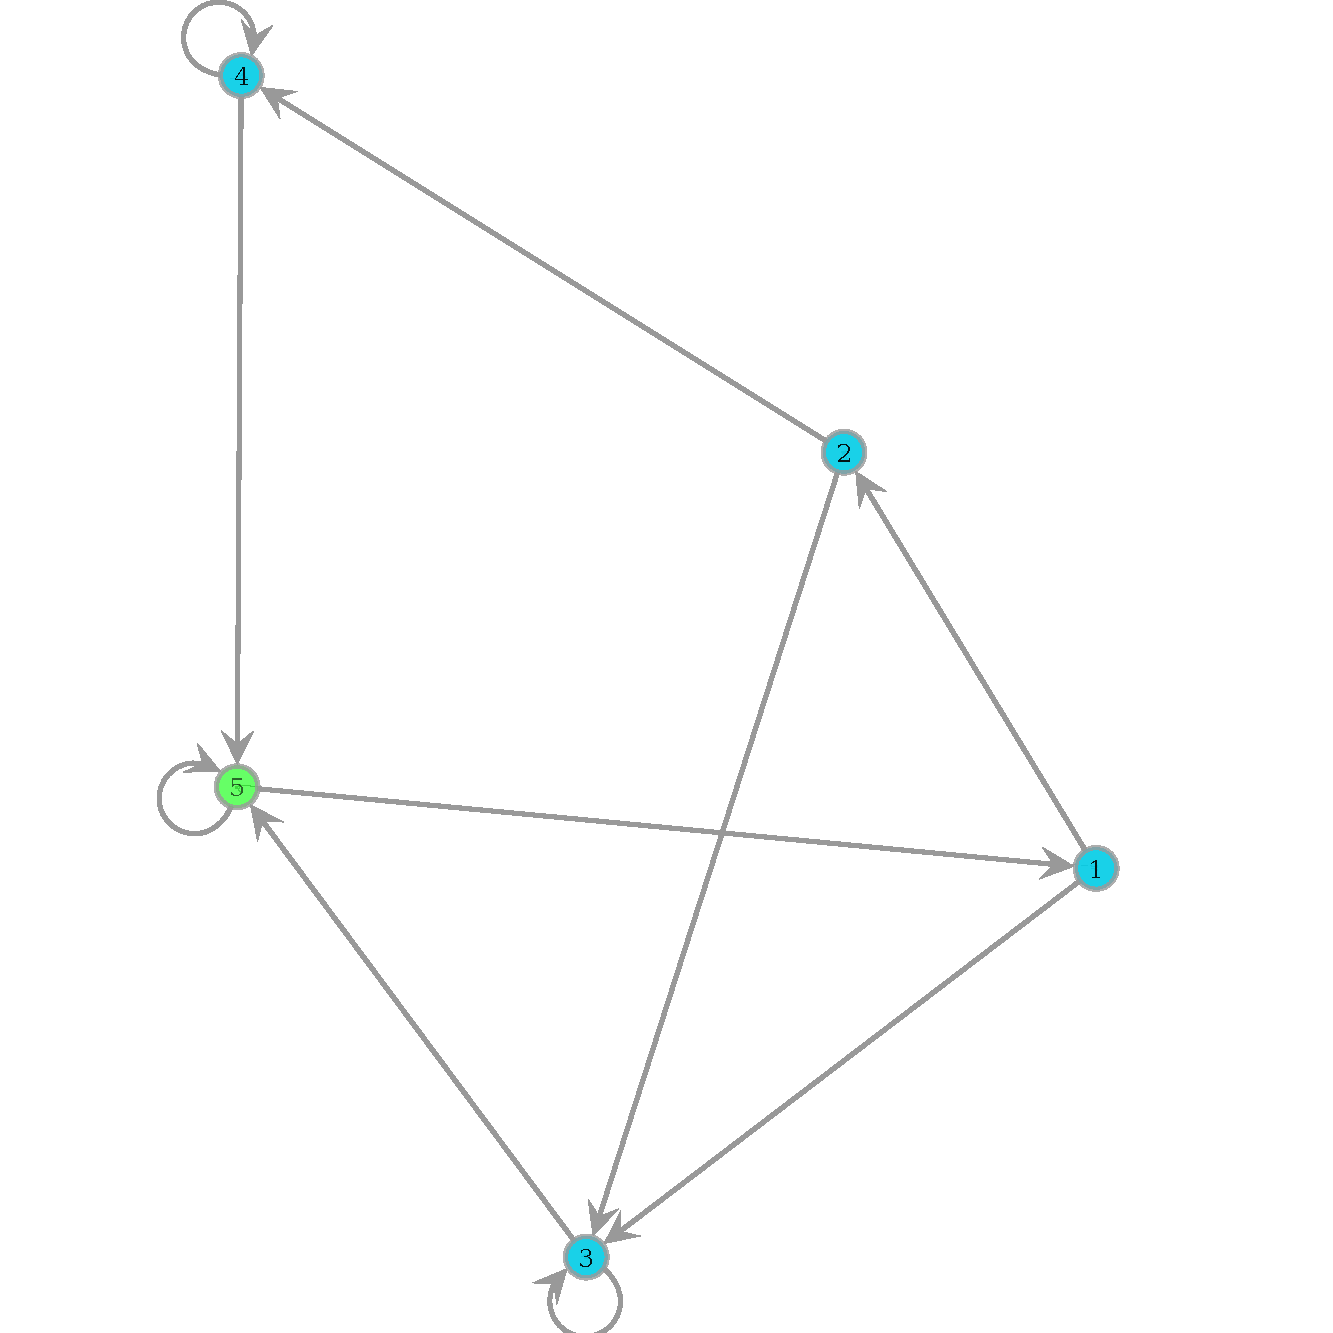
\includepdf[pages={1}]{mc_frame2.pdf}
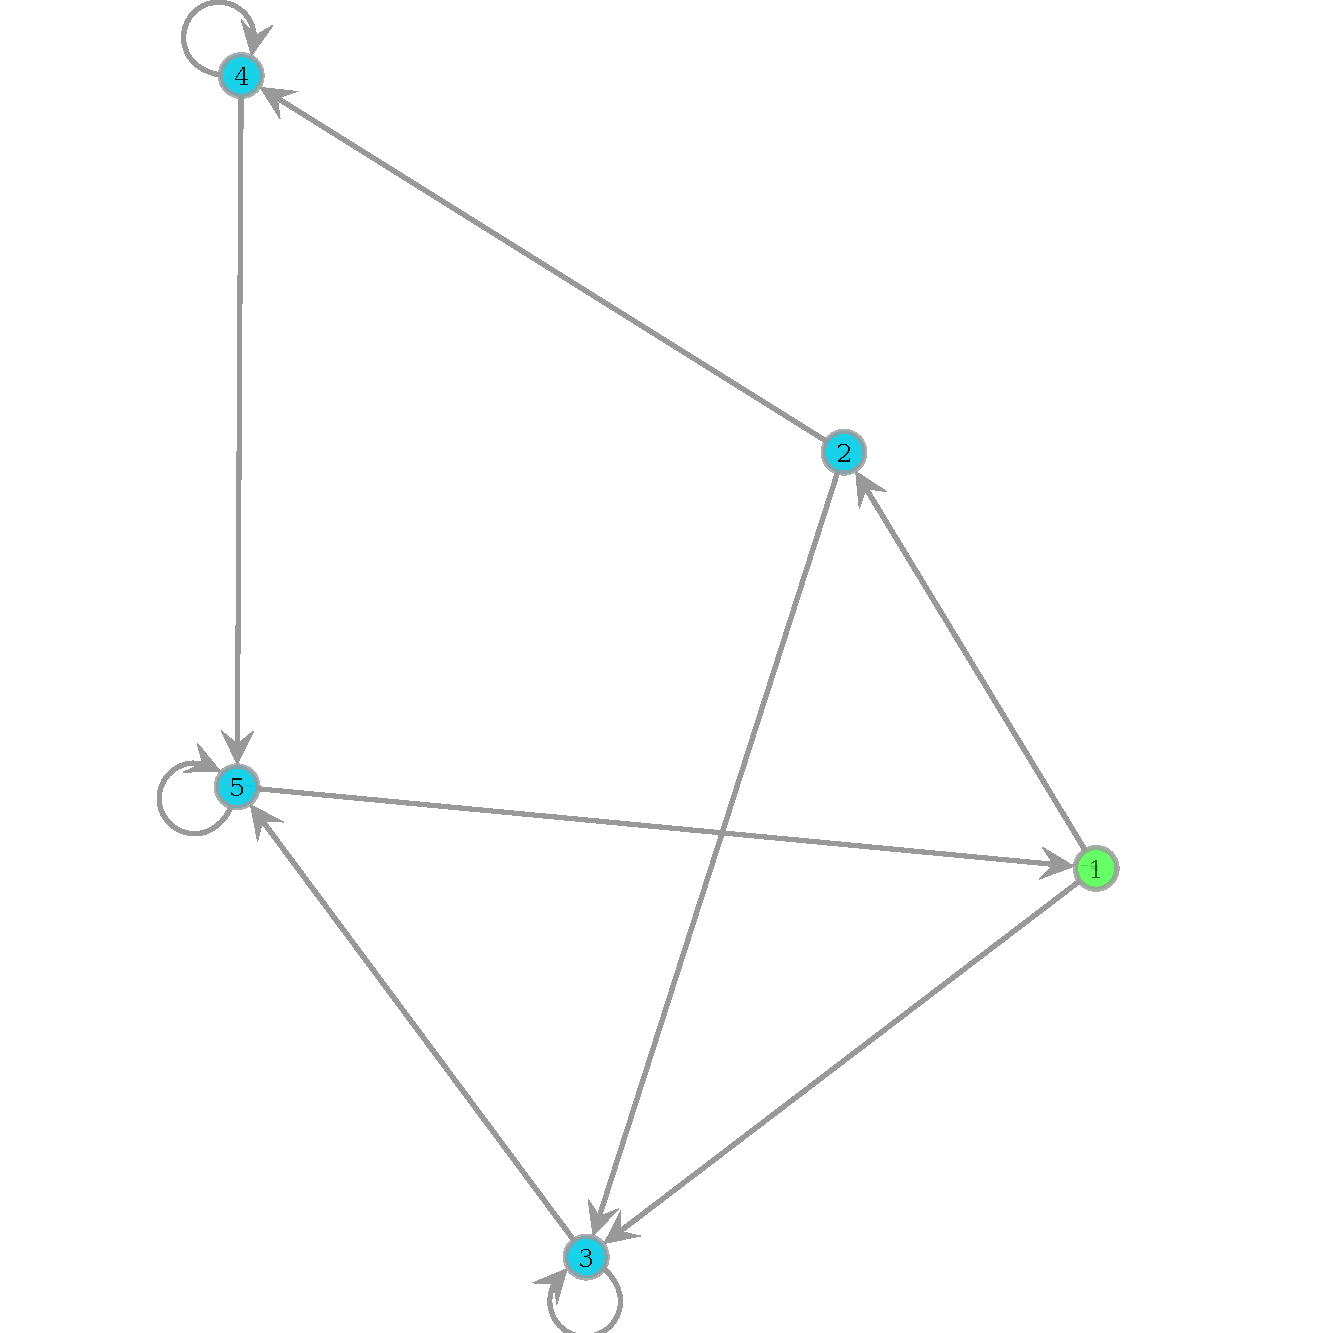
\includepdf[pages={1}]{mc_frame4.pdf}
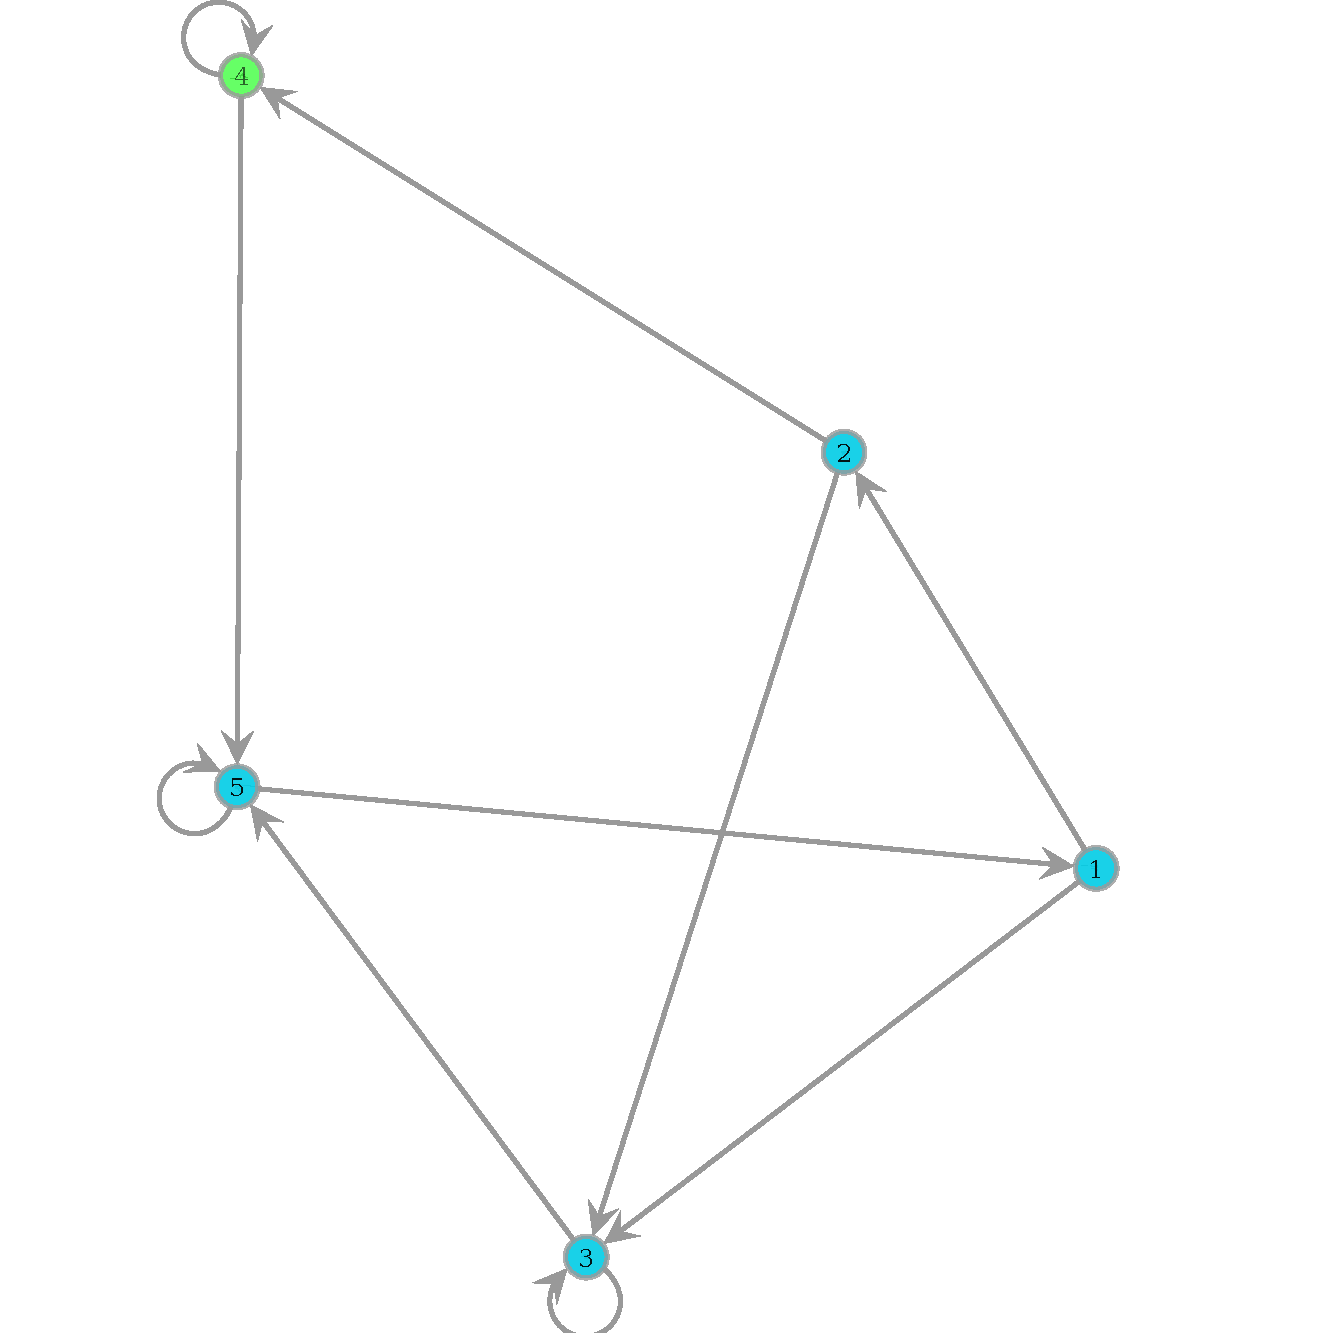
\includepdf[pages={1}]{mc_frame5.pdf}

\end{document}
